\input{../header.tex}

\subject{VERSUCH NUMMER 203}
\title{Verdampfungswärme und Dampfdruck-Kurve}
\date{
  Durchführung: DATUM
  \hspace{3em}
  Abgabe: DATUM
}

\begin{document}

\maketitle
\thispagestyle{empty}
\tableofcontents
\newpage
\setcounter{page}{1}
\section{Ziel}
\label{sec:Ziel}
\section{Theorie}
\label{sec:Theorie}

\subsection{Interferenz und Kohärenz von Licht}
Licht wird in diesem Versuch als elektromagnetische Welle betrachtet, um Interferenzerscheinungen erklären zu können. Die elektrische Feldstärke ist 
ebenfalls eine solche Welle und kann über 
\begin{equation*}
    \vec{E} = \vec{E}_0\cos{kx-\omega t - \delta}
\end{equation*}
beschrieben werden. Die Ausbreitung von Licht wird dabei über die Maxwellschen Gleichungen beschrieben. Außerdem folgt das elektrische Feld 
$\vec{E}$ dem Prinzip der linearen Superposition.
Die Intensität berechnet sich durch 
\begin{equation*}
    I = \text{const.}\cdot \rvert\vec{E}\lvert^2 \; .
\end{equation*}
Bei einer Überlagerung von zwei Wellen ergibt sich für die Intensität 
\begin{equation*}
    I = 2\cdot \text{const.}\cdot \vec{E}_0^2 \cos{\delta_2-\delta_1} \; .
\end{equation*}
Wenn die Bedingung
\begin{equation*}
    \delta_2 -\delta_1 = \left(2n+1\right)\pi 
\end{equation*}
erfüllt ist, ergibt sich die Intensität zu null.

Bei zwei unabhängigen Lichtquellen, sind die Phasenkonstanten $\delta_1$ und $\delta_2$ statistische Funktionen der Zeit, wodurch es keine 
Interferenzerscheinung gibt. Dieses Licht ist dann inkohärent. Mithilfe eines LASERs (light amplification by stimulated emission of radiation)
ist es jedoch möglich kohärentes Licht zu erzeugen, welches ein festes $k$, $\omega$ und $\delta$ besitzt.
Bei einem Wegunterschied der einzelnen Strecken des Interferometers, der der Kohärenzlänge $l$ oder mehr entspricht, verschwindet jedoch die 
Interferenzerscheinung. Die Kohärenzlänge berechnet sich über
\begin{equation*}
    l = \text{N}\lambda \; .
\end{equation*}
Dabei ist N die Anzahl der bei beobachtbaren Intensitätsmaxima. $\tau$ ist die Kohärenzzeit. 

\subsection{Das Michelson-Interferometer}
In \autoref{fig:michelson} ist der prinzipielle Aufbaue eines Michelson-Interferometers dargestellt. Dabei ist L die Lichtquelle, in diesem Fall
also ein LASER. P ist eine semipermeable Platte, die den Laserstrahl in zwei Lichtbündel aufteilt, sodass diese zwei verschiedene Strecken 
zu den Spiegeln $\symup{S_1}$ und $\symup{S_2}$ durchlaufen können. Beim zweiten Durchgang durch die semipermeable Platte werden die Strahlen 
wieder zusammengeführt und im Detektor D gemessen. 
\begin{figure}
    \centering
    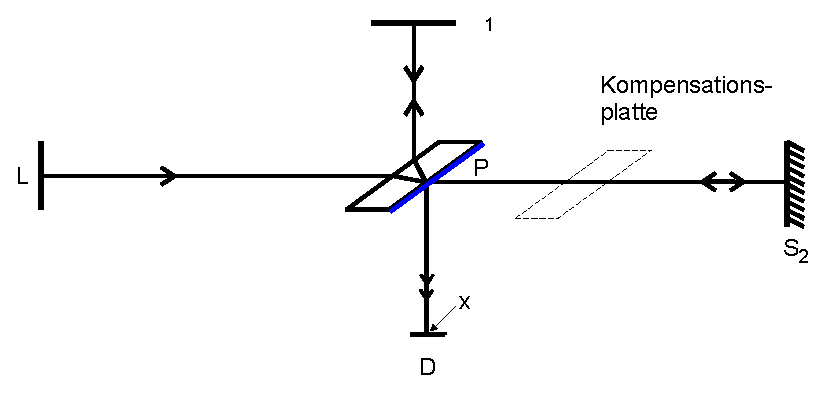
\includegraphics[height = 6cm]{michelson.pdf}
    \caption{Prinzipieller Aufbau des Michelson-interferometers \cite{ap401}.}
    \label{fig:michelson}
\end{figure}
Um Interferenzerscheinungen zu beobachten, muss das Licht kohärent sein, d.h. der Weglängenunterschied muss kleiner als die Kohärenzlänge $l$ sein. 
Aus diesem Grund wird er Abstand beider Spiegel gleich gewählt und eine Kompensationsplatte zwischen P und $\symup{S_2}$ eingebaut, sodass der längere 
Weg des Lichtstrahls zu $\symup{S_1}$ kompensiert wird. Wenn nun einer der Spiegel um $\symup{\Delta}d$ verschoben wird, ändert sich die detektierte 
Intensität. Es gilt
\begin{equation*}
    \symup{\Delta}d = z \cdot \frac{\lambda}{2} \; ,
\end{equation*}
wobei $z$ die Anzahl der Helligkeitsmaxima beschreibt.

\subsection{Bestimmung des Brechungsindex}
In \autoref{fig:mod} ist eine Modifizierung des Michelson-Interferometers dargestellt, bei der ein Medium der Länge $b$ in einen Strahlengang 
gesetzt wird.
\begin{figure}
    \centering
    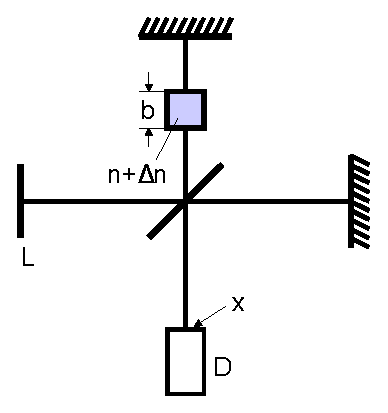
\includegraphics[height = 6cm]{modbrech.pdf}
    \caption{Modifizierung des Michelson-interferometers zur Messung des Brechungsindex \cite{ap401}.}
    \label{fig:mod}
\end{figure}
Der optische Wegunterschied ergibt sich damit zu 
\begin{equation*}
    b\symup{\Delta} = \frac{z\cdot\lambda}{2} \; . 
\end{equation*}
Durch die Dispersionsbeziehung ergibt sich für den Brechungsindex $n$
\begin{equation*}
    n = \sqrt{1+f\left(\lambda\right)\text{N}} \; .
\end{equation*}
Mit der idealen Gasgleichung, der Loschmidtschen Zahl $N_{\symup{L}}$ sowie einigen Umformungen kann der Brechungsindex über
\begin{equation*}
    n\left(p_0, T_0\right) = 1 + \frac{z\lambda T p_0}{2bT_0\left(p-p'\right)}
\end{equation*}
berechnet werden. 
%\section{Aufbau}
%\label{sec:Aufbau}

%Der schematische Aufbau der Messapparatur ist in \autoref{fig:mod} dargestellt. Es werden ein Laser, der kohärentes Licht abgibt, einen semipermeablen Spiegel, zwei Spiegel, einen Motor eine luftdichte Gaskammer und einen Detektor bestehend aus einem Phototelement, Signalverstärker und einem Impuslzähler.
%Die Bauteile werden wie in der Darstellung aufgebaut und so justiert, dass beide Teile des durch den semipermeablen Spiegel geteilten Strahls den Detektor exakt treffen. 
\section{Durchführung}
\label{sec:Durchführung}


\section{Auswertung}
\label{sec:Auswertung}

\subsection{Fehlerrechnung}
\label{sec:Fehlerrechnung}
Für die Fehlerrechnung werden folgende Formeln aus der Vorlesung verwendet.
für den Mittelwert gilt
\begin{equation}
    \overline{x}=\frac{1}{N}\sum_{i=1}^N x_i ß\; \;\text{mit der Anzahl N und den Messwerten x} 
    \label{eqn:Mittelwert}
\end{equation}
Der Fehler für den Mittelwert lässt sich gemäß
\begin{equation}
    \increment \overline{x}=\frac{1}{\sqrt{N}}\sqrt{\frac{1}{N-1}\sum_{i=1}^N(x_i-\overline{x})^2}
    \label{eqn:FehlerMittelwert}
\end{equation}
berechnen.
Wenn im weiteren Verlauf der Berechnung mit der fehlerhaften Größe gerechnet wird, kann der Fehler der folgenden Größe
mittels Gaußscher Fehlerfortpflanzung berechnet werden. Die Formel hierfür ist
\begin{equation}
    \increment f= \sqrt{\sum_{i=1}^N\left(\frac{\partial f}{\partial x_i}\right)^2\cdot(\increment x_i)^2}.
    \label{eqn:GaussMittelwert}
\end{equation}
\subsection{Auswertung der Messergebnisse}

Die Auswertung kann in zwei Teile unterteilt werden. Im ersten Teil wird die Wellenlänge $\lambda$ des Lasers bestimmt. Im zweiten Teil wird
der Brechungsindex von Luft untersucht.

\subsubsection{Berechnung der Wellenlänge des verwendeten Lasers.}
\label{sec:Wellenlänge}
Die 10 aufgenommenen Messwerte sind in \autoref{tab:Werte1} dargestellt. Aus jedem dieser Werte wird durch Umstellung von \autoref{eqn:Deltad} nach $\lambda$ ein Wert für die Wellenlänge bestimmt. 
Dabei gilt es zu beachten, dass bei der Berechnung der Hebelarm mit berücksichtigt werden muss. Um tatsächliche Verschiebung zu erhalten muss somit die gemessene Auslenkung mit dem Faktor $\frac{1}{5.046}$ multipliziert werden.% \textbf{oder Dividiert?????????}.
Aufgrund der Tatsache, dass während Messung 3 das Messgerät kurzzeitig ausgefallen ist, ist dieser Wert wesentlich geringer und wird deshalb weder in die Berechnung der Standardabweichung noch die des Durchschnitts der Wellenlänge einfließen.
Die Messgenauigkeit der Messschraube liegt bei $\pm 1.5\, \unit{\micro \meter}$\cite{Messgenauigkeit}. Dieser Fehler ist jedoch zum Ablesefehler, welcher sich auf $\pm 0.01\, \unit{\milli \meter}$ beläuft, nur etwa $15 \%$ so groß und deshalb vernachlässigbar.
Der Fehler der detektierten Maxima wird über die Standardabweichung errechnet. Hierzu wird \autoref{eqn:Standardabweichung} verwendet. Die Abweichung der Wellenlänge wird über die Gaußsche Fehlerfortpflanzung aus \autoref{eqn:GaussMittelwert} berechnet. 
\begin{table}
    \centering
    \caption{Messwerte zur Bestimmung der Wellenlänge $\lambda$}
    \begin{tabular}{c c | c}
        \toprule
        $d \mathrm{/} 10^{-3}\, \unit{\meter}$ & $z$: Anzahl der detektierten Maxima & $\lambda \mathrm{/} 10^{-9}\, \unit{\meter}$\\
        \midrule
        5.00 \pm 0.01 & 2540.00\pm 181.98& 780.22\pm 1.57\\
        5.00 \pm 0.01 & 2607.00\pm 181.98 & 760.17\pm 1.52\\
        5.00 \pm 0.01 & 2117.00\pm 181.98 & 936.12\pm 1.87\\
        5.00 \pm 0.01 & 3002.00\pm 181.98 & 660.15\pm 1.32\\
        5.00 \pm 0.01 & 2504.00\pm 181.98 & 791.44\pm 1.58\\
        5.00 \pm 0.01 & 2519.00\pm 181.98 & 786.73\pm 1.57\\
        5.00 \pm 0.01 & 2836.00\pm 181.98 & 698.79\pm 1.40\\
        5.00 \pm 0.01 & 2596.00\pm 181.98 & 763.39\pm 1.53\\
        5.00 \pm 0.01 & 2664.00\pm 181.98 & 743.91\pm 1.49\\
        5.00 \pm 0.01 & 2967.00\pm 181.98 & 667.93\pm 1.34\\
        \bottomrule
    \end{tabular}
    \label{tab:Werte1}
\end{table}
Aus den berechneten Einzelwerten kann so über \autoref{eqn:Mittelwert} und \autoref{eqn:FehlerMittelwert} ein Mittelwert und dessen Fehler beestimmt werden.
So ergibt sich für 
\begin{equation*}
    \bar{\lambda}_{\text{exp}}= (736.0\pm 1.5)\, 10^{-9}\, \unit{\meter}\, .
\end{equation*}


\newpage
\subsubsection{Bestimmung des Brechungsindex von Luft}
\label{sec:nvonLuft}
Der Brechungsindex wird mittels \autoref{eqn:brechung} berechnet und gemeinsam mit der Zählrate $z$ in \autoref{tab:brechung} dargestellt. Dabei wurden 
für die Normalbedingungen, die Temperatur und die Größe der Messzelle
\begin{align*}
    \text{Normaldruck: }p_0 &= 1.0132 \,\unit{\bar}\; ,\\
    \text{Druck: } p' &= (0.6 \pm 0.05) \, \unit{\bar} \; , \\ 
    \text{Normaltemperatur: }T_0 &= 273.15 \,\unit{\kelvin}\; ,\\
    \text{Umgebungstemperatur: }T &= 293.15 \,\unit{\kelvin}\; , \\
    \text{Größe der Messzelle: }b &= 50\,\unit{\milli\meter} \\
\end{align*}
angenommen. Auch hier wurde die Abweichung der Maxima mittels der Standardabweichung (\autoref{eqn:Standardabweichung}) berechnet, während die Abweichung 
der Brechungsindizes über \autoref{eqn:GaussMittelwert} berechnet wurde. 
\begin{table}
    \centering
    \caption{Messwerte zur Bestimmung des Brechungsindex $n$.}
    \begin{tabular}{c c}
        \toprule
        $z$: Anzahl der detektierten Maxima & $n$\\
        \midrule
        30 \pm 4.42 & $1.00058 \pm 7.04 \cdot 10^{-5}$\\
        17 \pm 4.42 & $1.00033\pm 3.99\cdot 10^{-5}$\\
        19 \pm 4.42 & $1.00037\pm 4.46 \cdot 10^{-5} $\\
        21 \pm 4.42 & $1.00041\pm 4.92 \cdot 10^{-5}$ \\
        24 \pm 4.42 & $1.00046 \pm 5.63 \cdot 10^{-5}$ \\
       
        \bottomrule
    \end{tabular}
    \label{tab:brechung}
\end{table}

Der Mittelwert des Brechungsindex ergibt sich zu
\begin{equation*}
    \bar{n} = 1.00043 \pm 0.00005 \; .
\end{equation*}
\section{Diskussion}
\label{sec:Diskussion}

Die ermittelte Wellenlänge hat den Wert $(736.0 \pm 1.5)10^{-9}\, \unit{\meter}$ und damit Abweichung von $(15.91 \pm 0.24)\%$ zum Theoriewert, welcher bei $635.0\cdot 10^{-9}\, \unit{\meter}$ liegt.
Die Abweichung könnte durch Verwacklungen der Apparatur oder durch das kurzzeitige Aussetzen des Messgerätes begründet werden. 
Durch einen vorsichtigeren Umgang mit der Messapparatur oder die Verwendung eines intakten Messgerätes könnte die Abweichung reduziert werden.

Bei der Messung des Brechungsindex  von Luft ist die sehr kleine Fehlerabweichung gegenüber des eigentlichen Werts bemerkenswert. Wenn dieser nun 
mit dem Literaturwert $n_{\symup{Luft}} = 1.0003$ \cite{brechung} verglichen wird, ergibt sich eine Abweichung von $0.01\,\%$. 
Da jedoch die Fehlerabweichung von $\bar{n} = 1.00043 \pm 0.00005$ ebenfalls sehr klein ist, liegt der Theoriewert nicht in dem Intervall. Somit stimmen die 
Werte von Theorie und Experiment nicht überein. Dies kann ebenfalls mit den oben genannten Gründen erklärt werden.

\newpage
\printbibliography
\nocite{ap308}
\nocite{matplotlib}
\nocite{numpy}
\nocite{scipy}
\nocite{uncertainties}
\nocite{reback2020pandas}

\newpage
%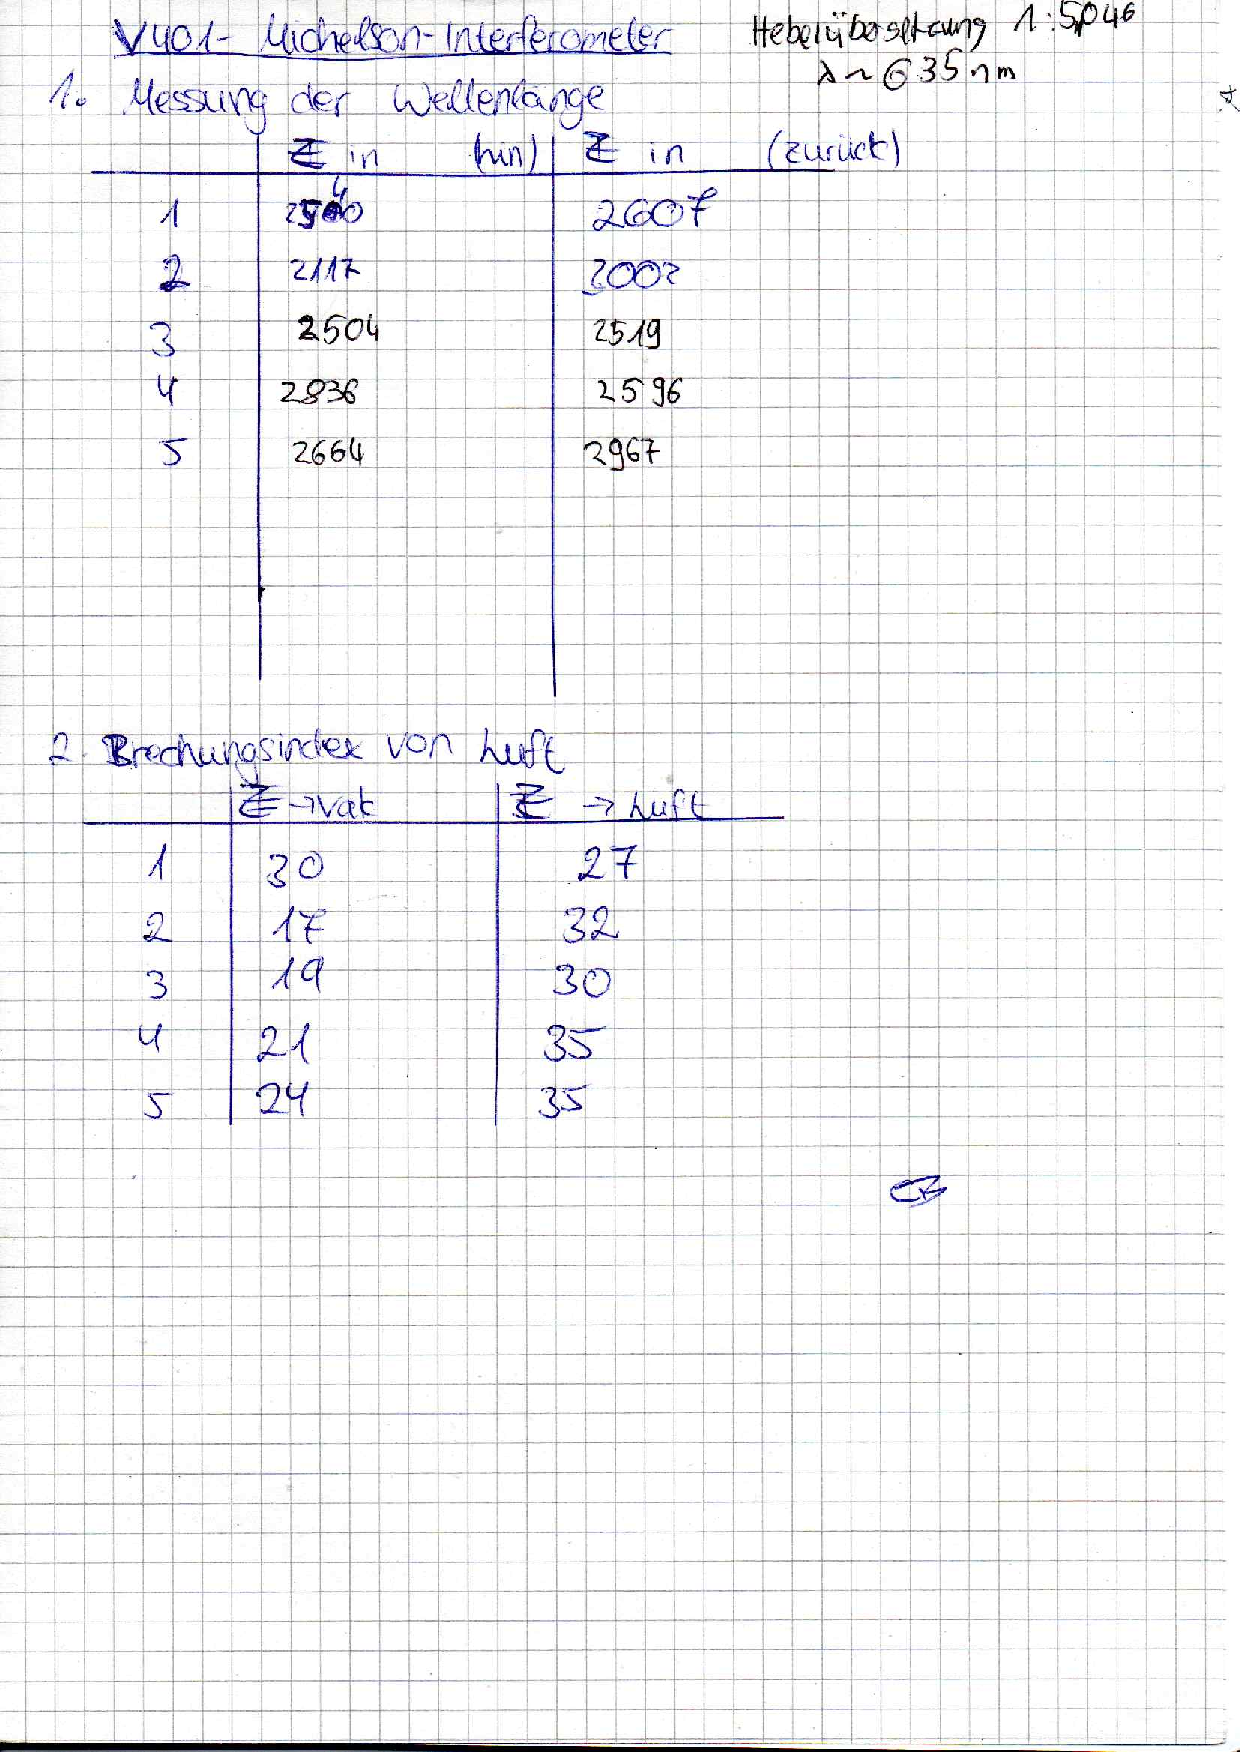
\includepdf[scale=0.9,pages=1,pagecommand=\section*{Anhang}\thispagestyle{empty}]{messdaten.pdf}
%\addcontentsline{toc}{section}{\protect\numberline{}Anhang}
%\includepdf[scale=0.9,pages=2-]{messdaten.pdf}
%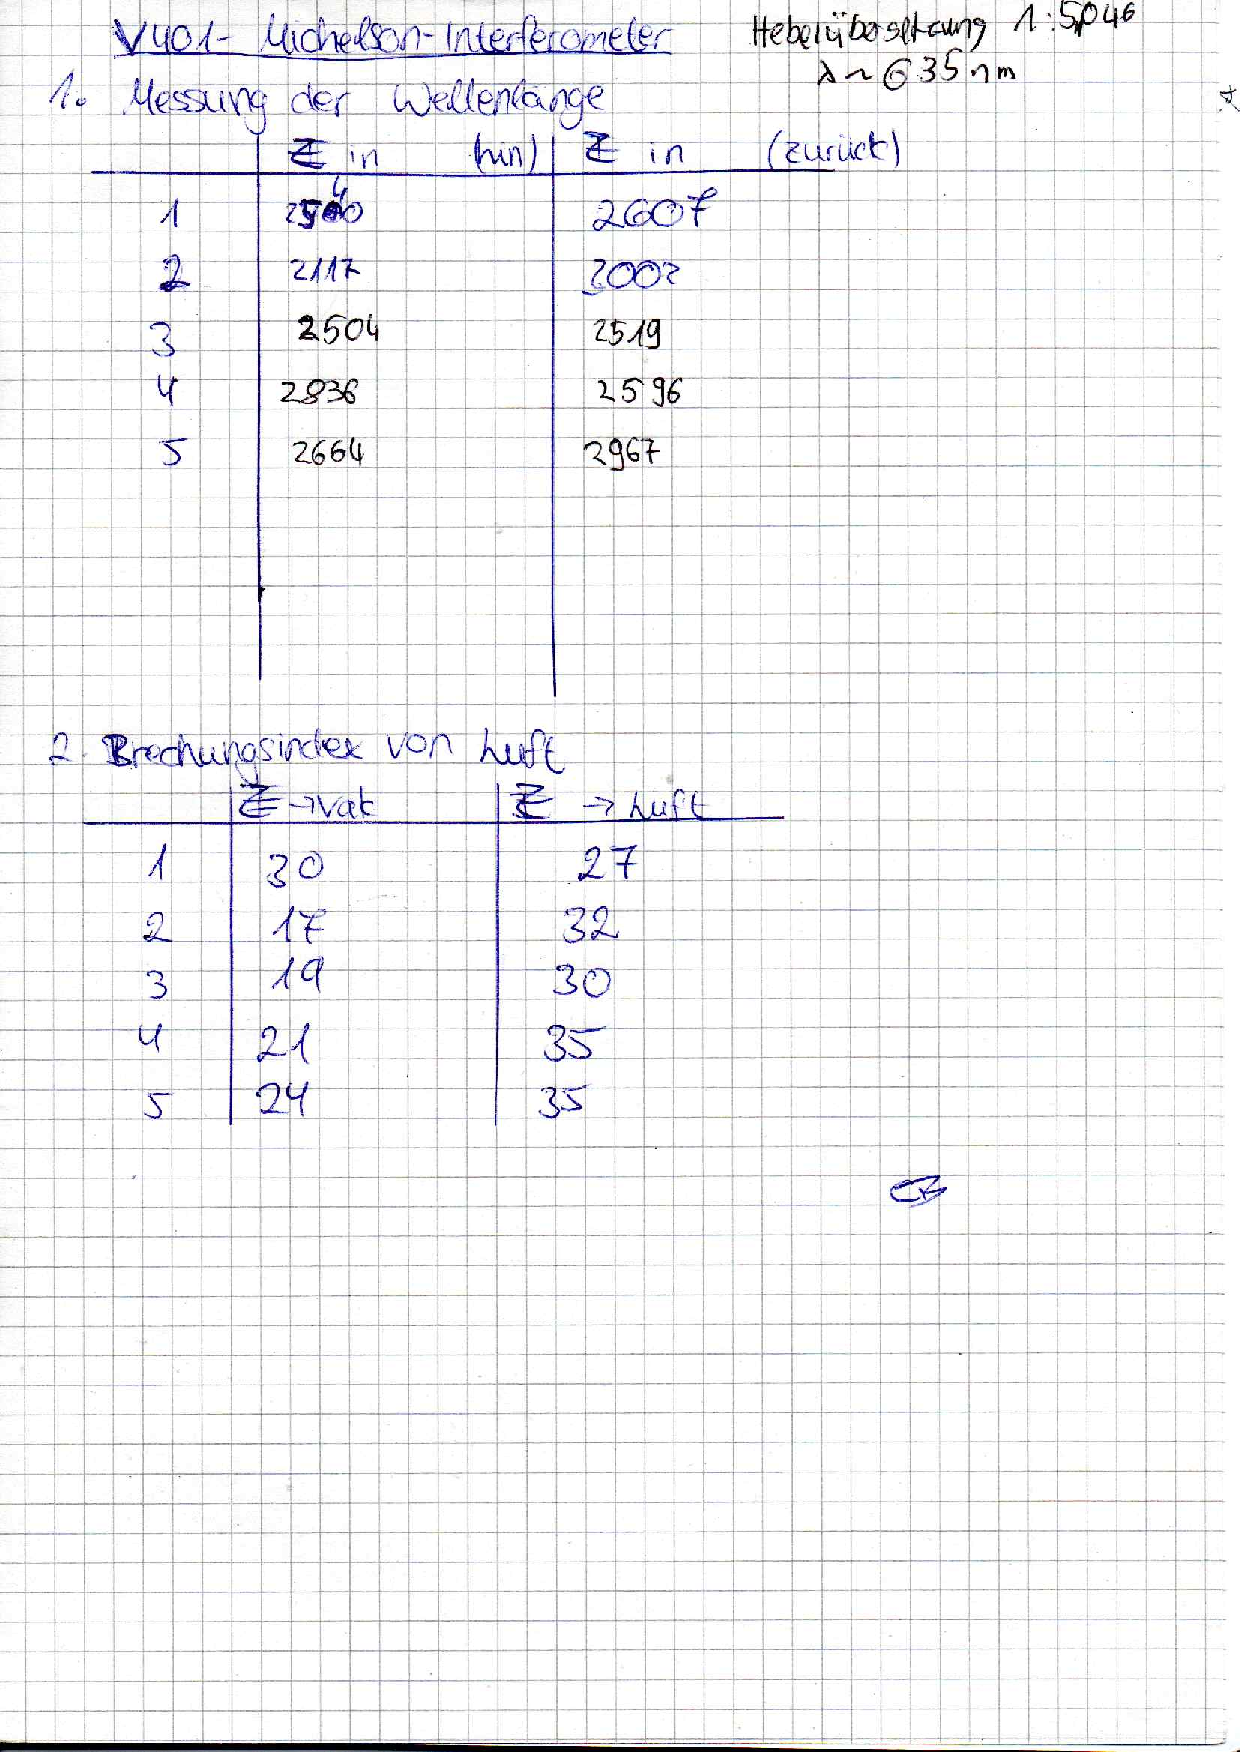
\includepdf[pages=-]{messdaten.pdf}

\end{document}
